\begin{refsection}

\chapter{Introduction}

Fusion energy is the way of the future, and to make the future a reality, the problem of confinement have to be solved. 
In order to produce net energy from fusion, the ion heat energy have to be sufficiently confined that the plasma could be maintained at the necessary high temperature without a need for excessive external heating. This requirement often expressed as the Lawson Triple Product:
\begin{align}
    nT\tau_{E} &\geq 10^{24} [eV m^{-3}s] &\text{  for T $\approx$ 15KeV D-T fusion.}
\end{align}
where n is the density, T is the temperature and $\tau_{E}$ is the energy confinement time of the D-T ions. Of the three values, the confinement time is the one that we have the least direct control over, and involves complex plasma behavior and interactions that needs to be better understood. A significant portion of fusion related plasma physics research involves the understanding, control and design optimization of confinement. A wide variety of confinement strategies area available, broadly separated into magnetic confinement and inertial confinement. Where as the inertial confinement focuses on short, repeated pulses of fusion reaction at very high densities typically driven by enormous lasers, magnetic confinement focus on using the magnetic field to restrict the movement of plasma particles long enough to produce net fusion power. 

\section{Ion transport in magnetically confined fusion plasmas}

Magnetic confinement fusion would ideally confine a volume of plasma in stable MHD equilibrium, while this plasma is fuled and heated to fusion conditions. However, physics mechanisms exist that would 'transport' energy out of the plasma even in such an equilibrium, limiting the confinement achieved. Transport mechanisms has been an important topic of study since the early days of fusion research. In general, transport in plasma are separated into what is called classical transport, neoclassical transport, and anomalous transport, with classical transport being the first order transport due to collisions, and the neoclassical transport from guiding center drift and toroidal magnetic geometry combined with collisions, and the anomalous transport referring to the transport that is observed but the mechanism of which is not clearly known. In more recent times, the anomalous transport have been strongly related to plasma turbulence, which leads to the term turbulent transport, which accounts for some or all of the anomalous transport. In parallel to the categorizations above, transport is also often separated into particle transport and thermal/heat transport, the former relating to the loss of particles, and the latter relating to the loss of thermal energy without necessarily losing the particles.
%Further, mechanisms relating to energy loss due to magnetic fluctuations or imperfect magnetic equilibriums are also included in the broader topic of transport studies.
\subsection{Classical transport}

Particles in a plasma undergoes collisions with each other, and in doing so, is able to diffuse across flux surfaces. In particular, the charged particles undergoes gyro-motion in the confining magnetic field and at random places during the gyro-orbit, undergoes Coulomb collision with another particle. In doing so, both particles involves are moved to new field lines resulting in particle diffusion. Alternatively, if two 'like particles' (\textit{i.e.} two deuterion, or two electrons) collide, they would result in no net motion, but thermal energy are exchanged. The diffusion of particles and heat due to this process is called classical transport, and will be addressed in section \ref{sec:thermal_cond}. In general, classical transport is small compared to other mechanisms, and scales favourably with temperature as collisionality will decrease.

\subsection{Neoclassical transport}

Neoclassical transport is also a collisional diffusion process, but it involves larger guiding center drifts and the orbits they result in. The toriodal magnetic geometry result in $\nabla\vec{B}$ drifts and curvature drifts off the flux surface. These drifts would average out during a complete poloidal orbit, but collisions before such an orbit is complete would result in the particle moving to, or exchanging heat with, another flux surface, which in turns leads to a diffusive process like the one for classical transport. Further, the toroidal geometry means that the magnetic field on the inboard side is necessarily higher than the outboard, leading to a magnetic mirror like 'experience' as particles traverse a poloidal orbit. Thus, a portion of particles are trapped by this effects and cannot complete poloidal orbit, but instead is trapped on the outboard side completing banana orbits due to the effect of the guiding center drifts. In the Tokamak geometry, the width of the banana orbit is large, and the collisional diffusion resulting from trapped particles result in transport significantly larger than classical transport. However, the RFP experiences very little neoclassical transport due to it's comparable poloidal B fields. Details of neoclassical transport, especially as it applies to the RFP, is discussed in section \ref{sec:neoclassical_cond}

\subsection{Turbulence and anomalous transport}

The observed transport often exceeds the predicted values from classical and neoclassical mechanism, and the difference is termed the anomalous transport. Studies have connected anomalous transport to the effects of plasma turbulence. Magnetically confined plasmas typically experiences magnetic turbulence as variable plasma oscillations and micro-instabilities propagate and interact in complex ways causing turbulent often stochastic motion. They are typically not able to be explain by near diffusion arguments and neither can they be calculated easily. Instead, the calculation of turbulent transport is the realm of sophisticated kinetic models, and multidimensional non-linear simulations, and our understanding of them are still incomplete. But great efforts are being made to quantify anomalous transport and significant progress is being made.

\subsection{Transport adjacent processes}

There are some transport mechanisms that do not fall neatly in the above categorization, the most important for the upcoming discussion is charge exchange losses. This refers to the energy lost due to ion-neutral collisions where an electron is exchanged causing the thermal ion to become neutral and lose confinement. Due to loss of confinement, a small amount of neutrals can have an out-sized effect on the evolution of ion temperature. As will be discussed more in detail in this work (section \ref{sec:neutral_physics} and \ref{sec:neutral_results}), the charge exchange process results in a warm neutral population of which a portion undergoes subsequent re ionization or charge exchange, in the process a portion of the lost energy is recovered to the ion fluid, making it a transport-like mechanism.

A similar situation applies to anomalous heating. Anomalous heating is known to be associated with sawtooth events in RFPs, where the sudden release of magnetic energy in due to reconnection and growing instabilities heats the ions. Such an effect is not transport in the sense that it is not moving energy around, or transporting them away. Although the instabilities certainly leads to increased particle transport, the anomalous ion heating itself is a energy source term that 'does work' on the ion fluid. But of course, in order to understand and predict the temperature in a plasma the anomalous source terms needs to be understood as well as transport. 

\section{The reversed field pinch and ion confinement challenges}

\begin{figure}[!htb]
	\centering
	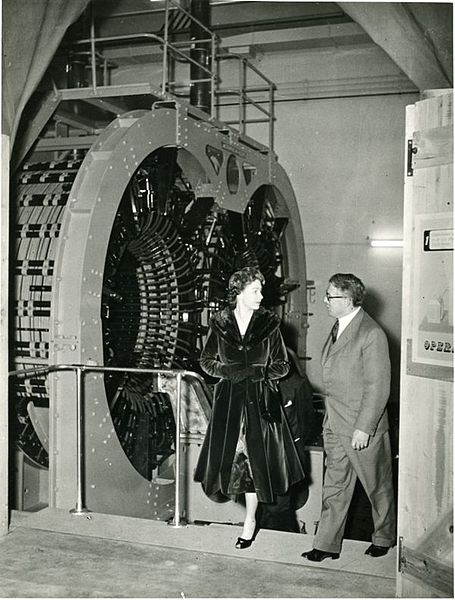
\includegraphics[width = 0.75\linewidth]{./1_Introduction/queen_at_zeta.jpg}
    \label{fig:Queen_at_ZETA}
    \caption[Queen Elizabeth II at the ZETA experiment]{Queen Elizabeth II of Canada visting ZETA during it's construction in 1957. Photograph by UKAEA}
\end{figure}%

The story of the reversed field pinch (RFP) starts with the Zero Energy Thermonuclear Assembly (ZETA). Initially built as an extension of the now abandoned toroidal pinch confinement concept, ZETA is one of the leading fusion experiment of its time. Scientists at ZETA discovered that spontaneous reversal of the magnetic field are associated with the most stable (quiescent) period of ZETA's plasmas \cite{Butt1966,Robinson1969}. This phenomenon was explained by J. Taylor in 1974 as a naturally result from the relaxation of the magnetic topology towards lower energy state \cite{Taylor1974}. These were the foundational documents of the RFP.

\begin{align}\label{eqn:helicity}
	K \equiv \int_{V} \vec{A} \cdot \vec{B} d\tau
\end{align}

Specifically, Taylor posited that in a toroidal plasma of finite resistivity constrained by a perfectly conducting shell, the magnetic helicity $K$ is conserved (eqn. \ref{eqn:helicity}). With this constraint, the plasma relaxes toward a state of minimum magnetic energy characterized by eqn. \ref{eqn:min_energy_condition}, where $\mu \varpropto K/ \Psi ^2$, is a constant unrelated to permeability . 

\begin{align}\label{eqn:min_energy_condition}
    \nabla \times \vec{B} = \mu \vec{B}
\end{align}

In cylindrical approximation, the solution to equation \ref{eqn:min_energy_condition} are Bessel functions (eqn. \ref{eqn:rfp_solution}) where $B_Z$ reverses in the edge if the plasma current is high compared to toroidal flux \cite{Taylor1974}.

\begin{align}\label{eqn:rfp_solution}
B_z &= B_0J_0(\mu r)\\
B_\theta &= B_0 J_1(\mu r)\\
B_r & = 0
\end{align}

The magnetic topology of atypical RFP is shown in figure \ref{fig:RFP_geometry}. The relatively low $B_t$ means the RFP have several advantages over the Tokamak. In the tokamaks, powerful toroidal field coils (TF coils) are used to generate toroidal flux and keep the safety factor q above 1 in order to stabilize the plasma. This leads to limits on the toroidal plasma current depending on the the available coil generated toroidal flux. This in turns is limited by engineering constrains in terms of magnetic coil construction. The reversed field pinch avoids these constrains, and
consequently can be constructed with much simpler and cheaper TF coil arrangements, as well as being more easily reach very high current levels to take advantage of large Ohmic heating, possibly to ignition levels.

\begin{figure}[!htb]
	\centering
	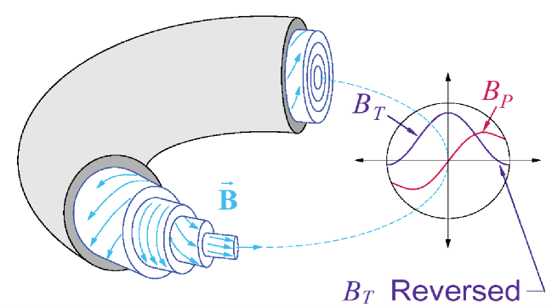
\includegraphics[width = 1.\linewidth]{./1_Introduction/RFP_mag_geometry.png}
	\caption[RFP magnetic topology]{Illustration of the RFP topology. The most distinct features of the RFP is the similar magnitudes of $B_t$ vs. $B_p$, as well as the fact that $B_p$ reverses direction near the edge.}
	\label{fig:RFP_geometry}
\end{figure}%

However, the magnetic topology also poses challenges to the RFP's confinement characteristics. Taylor noted that the relaxation of the magnetic field is made possible by the finite resistivity, but did not speculate on the 'method' of
relaxation. Experiments have shown that the relaxation occurs via resistive tearing mode instabilities which poses a challenge to RFP confinement characteristics.

\begin{figure}
	\centering
    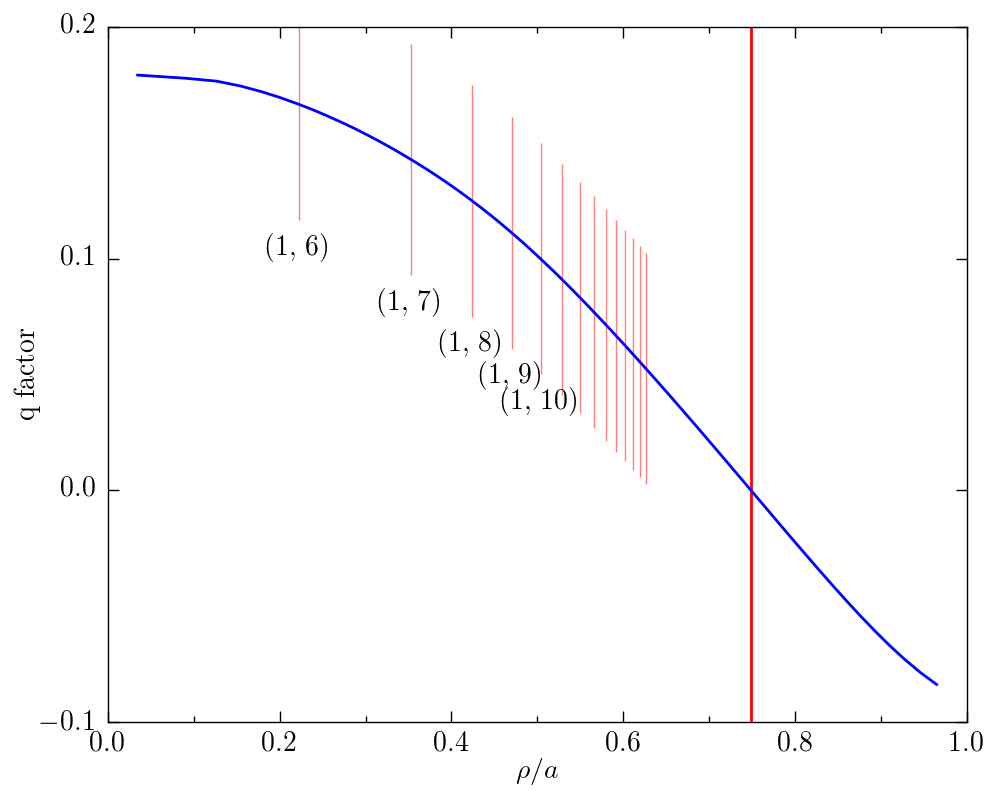
\includegraphics[width = 1.\linewidth]{./1_Introduction/PPCD_q_profile.png}
    \caption[Example RPF q profile]{q profile typical of the plasmas studied in this work. Note the closely space resonant surfaces near the reversal surface. These plasmas have a deeper reversal than standard RFP operation due to the confinement improvement techniques explored in the next chapter.}
    \label{fig:q_profile}
\end{figure}

The finite resistivity of the plasma allows for the reconnection of the magnetic field lines and the formation of magnetic islands through tearing mode instabilities. Tearing modes are unstable at magnetic resonant surfaces where the safety factor $q \equiv \frac{rB_T}{R_0B_p}$ is a rational number, ie $q = \frac{m}{n}$ where m and n are integers. The location of these unstable regions form 'resonant' surfaces that are typically labeled by their m and n numbers. The RFP have q lower than 1 everywhere, and further decreases monotonously towards the edge where it will cross 0. An example q profile is show in figure \ref{fig:q_profile}. This leads to the existence of a large number of resonant surfaces, especially close to the reversal surface. 

These closely spaced resonant surfaces and the tearing mode instabilities that they 'host' creates regions of overlapping magnetic islands that turns the magnetic field stochastic, greatly reducing the confinement characteristics. The primary drive of the tearing mode instabilities are the current density gradient\cite{Schnack1987,Ho1991}. Specifically $\nabla\lambda$ where,
\begin{align}
    \lambda &= \frac{J_{\parallel}}{B}\\
    &= \frac{\vec{J}\cdot\vec{B}}{B^2}\nonumber
\end{align}
where $J$ is current, $B$ is magnetic field, and all quantities are flux surface averages. In standard RFP operation, the $\lambda$ profile tends to peak in the core of the plasma as the result of current drive, providing free energy to core resonant tearing modes. As the current peaks, the core tearing modes grow and non-linearly couples to each other, until they are sufficiently large to trigger a violent relaxation event called a sawtooth crash. This redistributes the current profile such that toroidal current in the core decreases while the poloidal current in the edge increases\cite{Terry2004}. This effectively flattens the $\lambda$ profile and decreases the drive of the tearing instabilities. But the process repeats as the current profile peaks again in a cycle that is referred to as the sawtooth cycle. Though ion heating is observed with the sawtooth crashes\cite{Bodin1980}, they greatly decreases confinement and is undesirable for fusion development.

\section{Improving confinement with inductive current profile control}

One successful way of improving confinement on the RFP, therefore, is through the control of $J_{\parallel}$ profile. This is done inductively on MST through a process called Pulsed Parallel Current Drive (PPCD). PPCD can be thought of as 'helping' the plasma to drive parallel current in the edge region, and thereby flattening the $\lambda$ profile\cite{Sarff1995}. In particular, a series of 4 high voltage capacitor banks discharges are used to apply voltage to the toroidal field circuit. This result in a series of 4 poloidal field pulses, which raises $E_{\parallel}$ in the edge. Thus, PPCD is a transient current drive and profiles of the RFP continually evolve during this period. 

With successful applications of PPCD, sawtooth cycles are interrupted which allows a new class of dynamo events called m = 0 bursts to come to the forefront. Details regarding these m=0 bursts are discussed in chapter \ref{ch:m0}. In the meantime it suffice to say that the frequency of these m=0 bursts can be significantly reduced by reversing the applied toroidal electric field in the edge of the plasma\cite{Chapman2001}.

\begin{figure}
    \centering
    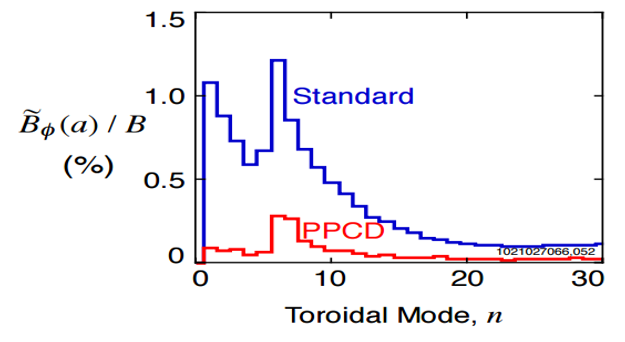
\includegraphics{./1_Introduction/ppcd_fluc.png}
    \caption[Typical tearing mode amplitude in PPCD]{Typical tearing mode amplitude in PPCD.}
    \label{fig:ppcd_fluc}
    %TODO: consider remaking this plot for my particular plasmas if time allows
\end{figure}

PPCD reduces the tearing mode fluctuation levels significantly as shown in figure \ref{fig:ppcd_fluc}, and during the period of improved confinement, $T_e$ is known to increase dramatically as compared to standard MST plasma, while $T_i$ is observed to be relatively flat, resulting in temperature differences as high as $T_e \approx 2T_i$ in the core of the plasma. At the same time, recent observations shows that drift wave turbulence, likely associated Trapped Electron Mode, continues to be present in PPCD plasma in the edge. 

Though the electron transport properties in PPCD have been studied as part of several thesis previous, the ion transport, particularly the ion thermal transport has not been studied in the same detail. This has hampered past efforts at studying anomalous heating that results from sawtooth events. Characterizing ion thermal transport dynamics in the RFP would help establish a baseline for investigation of more complex heating phenomenons, in addition to the inherent value of understanding the ion thermal transport itself, and the identification of key energy loss mechanisms.

\section{What this thesis is about: 1-D classical transport modeling}

This thesis project aims to characterize the ion thermal transport in MST during the improved confinement periods achieved through PPCD. It approaches this question by the construction of a 1-D model of thermal transport that makes predictions on ion temperature evolution from an initial condition and diagnostic measurements of plasma parameters, with exception of $T_i$ itself. The model prediction are them assessed by comparing with measurements. The model considers classical collisional mechanisms, with addition considerations for charge exchange and flow, and unlike some similar assessments previously performed, it is not an equilibrium power balance calculation (\textit{i.e.} $\partialt x \approx 0$ for relevant parameters). Instead, at it's core, it is a foreword model based on a numerical integration of the following equation in time,
\begin{align}
    \partialt E_\text{thermal} = P_\text{e-i} + P_\text{cond} + P_\text{CX} + P_\text{flow} + P_\textit{ad hoc}
\end{align}
where the different $P$ terms denotes thermal power terms acting upon majority ion fluid, and are functions of time and $\rho_v$, the radial coordinate. This equation is revisited in more detail in section \ref{sec:transport_summary}, after the details of the terms are discussed. 

The thesis starts in chapter 2 by discussing the various physics mechanisms included in the model as well as the consideration for those that are not. Chapter 3 gets into the details of the hardware and diagnostic used to calculate the model terms, as well as considerations for the implementation and coding strategies used in the model. Chapter 4 details discoveries made working with the model analysis, including about neutrals and flow in the plasma, then discusses modeling results and comparisons to measurements, as well as the need for an \adhoc term in the edge. Chapter 5 discusses the adjacent topic of impurity heating observations during m = 0 bursts, a reconnection phenomenon that sometimes occurs during PPCD periods, following by chapter 6, a short summary of the results and directions for future work.

\begin{figure}
    \centering
    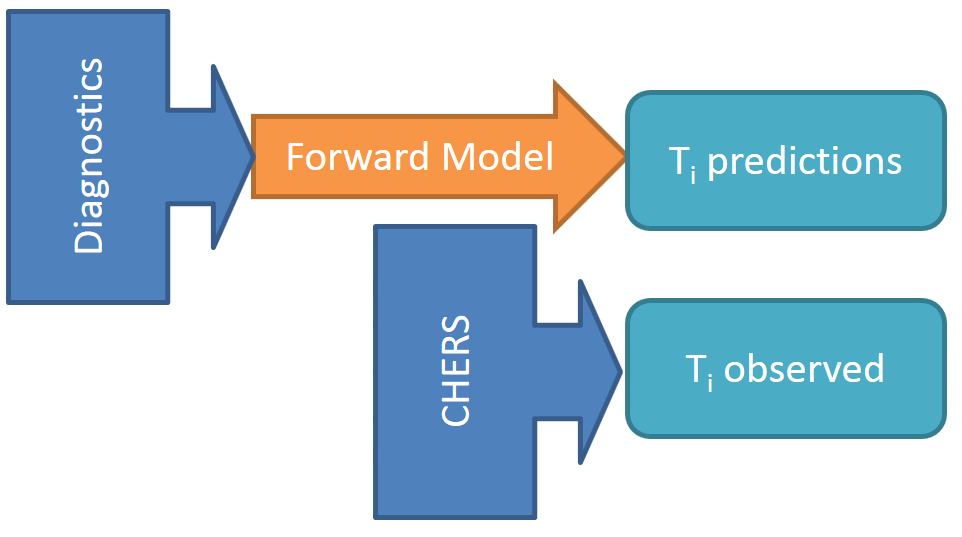
\includegraphics[width=0.75\linewidth]{./1_Introduction/exp_structure_diagram.png}
    \caption[Block diagram of experiment]{Block diagram of experiment.}
    \label{fig:ppcd_fluc}
    %TODO: consider remaking this plot for my particular plasmas if time allows
\end{figure}

\printbibliography


\end{refsection}